\chapter{Csónak}

\keywords{sétáló meditáció módszere}

\noindent A sétáló meditáció egy energikusabb alternatíva az ülő
testtartás mellett. Keress egy ösvényt, vagy egy kis területet, ahol van
elég hely megtenni néhány lépést, oda-vissza séta közben. Habár
sétálunk, a figyelmünket befelé irányítjuk. Nem egy bizonyos helyre
sétálunk. A sétáló testtartást használjuk az elme fejlesztésére.

Egy kültéri, magányos helyszín az ideális, de beltérben, egy nagyobb
szoba is megfelelő.

Válassz két pontot, ami között tisztán járható út van. Ez lehet két fa,
vagy akár két bútor is. Egy rövid ösvény vehető tizenöt lépés hosszúnak,
egy hosszabb lehet harminc lépés is. Állj meg az ösvény egyik végén, és
indulj el lépésenként, figyelmesen a másik végéhez, tisztán elhatározott
szándékkal arra, hogy a meditáció tárgyával maradsz, mint például a
lélegzet, vagy a mozgó test fizikai érzetei. Irányítsd a tekinteted
lefelé, nézz magad elé néhány lépésnyire. Az ösvény másik végén állj
meg, és várj pár lélegzet vételnyi időt. Tartsd a figyelmed elmélyedve a
meditációban, fordulj meg, és kezdj el sétálni a másik irányba.

Tartsd a kezed úgy, hogy segítsen fenntartani a folyamatos belső
figyelmet. A legtöbben összefogják a két kezet maguk előtt. Nem a kezek
pontos helyzete számít, de ha oda-vissza lengeted a karjaid, az könnyen
eltereli a figyelmed.

\clearpage
\thispagestyle{empty}\mbox{}
\photoFullBleedPlaceholder{%
  TODO: Illustration of walking meditation.%
  \illustration{Sétáló Meditáció Testtartás}%
  \label{illus-walking-meditation}%
}
\clearpage

Igazítsd a séta sebességét az energia szintedhez és a meditáció
tárgyához. Egyesek gyors és határozott lépésekkel gyakorolják a sétáló
meditációt, mások lassú és óvatos lépéseket tesznek. A megfelelő
sebesség akár egy alkalom időtartamán belül is változhat. Tapasztald meg
a különféle változatokat és találd meg azt, ami illeszkedik a
gyakorlásodhoz és mentális hátteredhez az adott helyben és időben.

\keywords{az érzések manipulálása, fontoskodás}

Korábban, a sétáló meditációtól csak még feszültebb lettem. Úgy
gondoltam hasznos, de a módszer elég határozatlan volt, és nem voltak
pontos részletek arról, hogyan is kellene azt végezni. Úgy éreztem, egy
pontokba szedett listára van szükségem, amin végig mehetek és
ellenőrizhetem, jól végzem-e a feladatot vagy sem.

Folyton el akartam sétálni egy \emph{másik helyre}, ahol majd
\emph{máshogy érzem} magam. Elkezdtem a sétáló meditációt két fa között,
de úgy éreztem mintha nem lenne semmi hatása, és folyton változtattam a
séta módját, hogy manipulálni tudjam hogyan érzem magam. `Lépkedj
gyorsabban, az használni fog. Lassíts le, és összpontosíts. Próbálj így
lélegezni, és úgy lépkedni, amíg máshogy nem érzed magad.'

Az is fontos volt, hogy mások lássák, valami fontos dolgot csinálok.
Addig járkáltam oda-vissza, amíg a füvön elkezdett látszódni a
kitaposott ösvényem. Ez volt a bizonyíték: 'Itt van, látom, hogy tettem
valamit, és \emph{mások} is láthatják!

Látható, hogy az ilyen küszködést mennyire az a kérdés vezérli: `Hogyan
tudnám jobban érezni magam, magammal kapcsolatban?'

A motiváció az érzések \emph{manipulálása} körül forog, nem azok
\emph{megértését} keresi, hogyan keletkeznek és múlnak el. A fontoskodás
nem hasznos hozzáállás a gyakorláshoz. A vágyunk meghatároz egy külső
jelet, és szörnyen fontossá válik, hogy ezt lássuk, és, hogy mások
számára látható legyen. Az a \emph{fontos} ösvény a fűben amit a fűbe
tapostam (ami valószínűleg eltűnt a következő reggelre) egy példa erre.
Kifejezni ezt a magunk számára, amikor észrevesszük, hogy ez történik,
már önmagában megváltoztatja a hozzáállásunkat a folyamathoz.

Egy hasznos hozzáállás a gyakorláshoz az, ha úgy közelítjük meg, mintha
valami teljesen hétköznapi dolgot végeznénk, de ehhez hozzáfűzzük a
felfedezés szemléletét, és emlékezünk arra, hogy az értéke nem egy
világi cél, ebben nincs tét, amit megnyerjünk, vagy elveszítsünk. Az is
segíthet, ha \emph{csökkentjük} a meditáció idejét. Jó benyomást kelt,
ha három óra hosszat folyamatosan sétáló meditációval töltünk, de a
nyomás feszültséghez vezet. Mi a helyzet tíz perc meditációval? Lehet,
hogy nem világhír, de talán jó élmény és érdekes lesz.

\keywords{gondolatok megállítása, éberség a fejben, belső monológ, irányítás, hétköznapi gyakorlás}

A gondolkodás jellemzően erősödik és önmagunk körül forog, amikor úgy
tekintünk az éberségre, tudatosságra, vagy a meditációra, mint egy olyan
dologra, ami valahol a fejünkben történik. Abból a nézőpontból, az
éberség olyan dologgá válik, amit `nekem kell csinálnom az
agyamban'.\footnote{Cf. Chapter 4, `Mindfulness Mania' in
  \href{https://www.goodreads.com/book/show/44439993-why-i-am-not-a-buddhist}{Why
  I Am Not a Buddhist by Evan Thompson}} Ez alá becsüli az éberséget,
mintha csupán egy rongybaba lenne az agy bábszínházában. Habár ez a kép
illik a kedvenc elképzelésünkhöz, ami szerint mi irányítjuk a műsort, ez
a valóság egy szűk nézete.

A kognitív felfogásunk ennél egy sokkal összetettebb, a környezetet
magába foglaló folyamatok rendszere. Megfigyelheted, hogyan változik a
figyelmed, vagy az egész személyes hozzáállásod, például amikor egyik
épületből belépsz a másikba, vagy a belső térből a szabadba. A tested
reagál arra, hogy egy új környezetben vagy, a különféle szociális
környezet megváltoztatja a viselkedésed, nagyszámú belső és külső
tényezők vesznek részt abban, hogy létrehozzák az észlelést, amit úgy
tapasztalsz mint `az én elmém.' A felfogásunk, vagy elménk, magába
foglal egy hálózatban működő folyamatok együttesen működő rendszerét,
melyek a testünk széles környezetéből veszik a beérkező jeleket. Ahogy
többet tapasztalunk ebből történés közben, az derül ki, hogy nincsenek a
kezünkben a drótok, amiket meghúzva az elménk akaratunk szerint járja a
táncot.

A gondolkodó és érvelő elme egy eszköz, amit a minket motiváló célokra
használunk. Nem a `jó érv' motivál minket, hanem a motiváció miatt
keresünk jó érvet. Ne akarj a gondolatok végére jutni; vedd észre mi az,
ami motivál téged a gondolkodásra. Ha azt elengeded, a gondolkodást is
elengeded. A belső rágódással gyakran magunkat akarjuk vigasztalni úgy,
hogy elképzeljük, mintha lenne irányításunk egy bizonyos helyzetben;
vagy megpróbáljuk visszanyerni az irányítást valami olyasmi felett, ami
már megtörtént. Olyan ez, mintha az esőről gondolkodnánk: esni fog attól
függetlenül, hogy rágódunk rajta vagy sem.

Ha \emph{tudunk} tenni valami hasznosat a problémával kapcsolatban, az
megnyugtató. Ha nem tudunk, mert teljesen az irányításunkon kívül esik,
legalább ezt tudhatjuk, és felhagyhatunk a belső tépődéssel.

A gondolkodásnak gyakran egy élesen meghatározott szóbeli tárgya van.
Amikor a figyelmünk módját eltoljuk egy tágasabb, folyékonyabb
hozzáállás felé, az elme nem tud szavakat találni rá, és átváltunk egy
nem verbális, szótlan felfogási módba; a körülöttünk lévő világot ezen
keresztül észleljük.

A nem-gondolkodás úgy tűnhet mint valami misztikus állapot, mintha egy
magas fokú meditációs szint lenne. Nem szoktuk megkérdezni meditáló
társainktól mennyi belső párbeszédet használnak, ugye? Amikor
megkérdezzük az embereket, kiderül, hogy van aki egyáltalán nem folytat
magával belső monológot.\footnote{\href{https://www.psychologytoday.com/us/blog/pristine-inner-experience/201110/not-everyone-conducts-inner-speech}{Not
  Everyone Conducts Inner Speech (psychologytoday.com)}} Sokkoló
meglepetésként éri őket, amikor megtudják, hogy más emberek beszélnek
magukkal a fejükben. Mások csak időnként kezdenek belső párbeszédet, míg
megint mások folyamatosan, szünet nélkül ezt teszik. Ez egy érték skála,
mint egy tekerő gomb különféle állapotai. Személyesen hozzá vagyunk
szokva egy bizonyos mértékű belső párbeszédhez, de a szint, amin ezt a
mentális képességet használjuk egy szokás, amin állítani tudunk.

Ha séta közben úgy érzed, magával ragadott a gondolkodás, vedd tágabbra
a területet, amire tudatos vagy; hogy magába foglaljon egy szélesebb
kognitív mezőt. Idézd fel a nyugodt hallgatás hozzáállását, fordítsd el
a figyelmet a szemek és a fej környékéről más irányba.\footnote{Cf. page
  117, Gently Listening in
  \href{https://forestsangha.org/teachings/books/alert-to-the-needs-of-the-journey?language=English}{Alert
  to the Needs of the Journey by Ajahn Munindo (forestsangha.org)}}
Tartsd a szemeket magad előtt, alacsonyan a sétáló ösvényen.
Képzelheted, mintha minden irányba látnál a testeddel, vagy mintha az
ösvényt a talpaidon keresztül látnád, a tapintás és nyomás érzetein át.
Nyisd meg a figyelmed, hogy magába foglalja az egész testet, mint
egyetlen mozgásban lévő érzet. Nyisd a figyelmet még tovább, ki a sétáló
ösvény közvetlen környezetére.

Rövid meditációk, amik betöltik a céljukat, jobbak, mint hosszú
időszakok, amit azzal töltesz, hogy az óra állásán aggódsz. A cél nem
az, hogy több feszültséget keltsünk. A cél az elme tisztán látása és
nyugalma. Gyakorolunk, vele maradunk, így élünk abban a térben, ahol a
feszültség feloldódik.

\keywords{a tapasztalatok figyelése, érzékek kontaktusa}

A meditáció elején összegyűjtjük a figyelmünket azzal, hogy a légzést
figyeljük, vagy a séta közben tapasztalt érzéseket, lépésről lépésre.
Egy zaklatott, izgatott elmétől nem várhatunk éber és kiegyensúlyozott
intelligenciát, ezért lényeges megalapozni legalább némi nyugalmat.

Vizsgálódásra a nyugodt elme alkalmas. Mit tanulhat a boldog ember a
Buddha tanításából? Mit tanulhat a boldogtalan ember? Vagy, aki nem érzi
magát sem különösen jól vagy rosszul, éppen megvan ahogy van?

A tapasztalatunkat figyeljük, az állandótlanság jeleit, az érzések,
gondolatok kezdetét és végét, ahogy megjelennek, változnak és
megszűnnek. A magunk számára vizsgálódunk, ez ad a tanítások szavainak
jelentést és közvetlen hasznot.

Tapasztalataink az érzékeken keresztül nyilvánulnak meg. A szem formákat
és színeket fog fel, a fül hangokat, az orr szagokat, a nyelv ízeket, a
test a tapintás, a hideg és meleg benyomásait érzékeli, az elme pedig
észleli a gondolatokat, emlékeket és más mentális folyamatokat.

\keywords{három érzés, állandótlanság}

Az érzetek (\emph{vedanā}) három minőségben jelennek meg. Lehetnek
kellemesek, és vonzódunk feléjük; lehetnek kellemetlenek vagy
fájdalmasak, és inkább távolodnánk tőlük; vagy lehetnek semlegesek, és a
jelenlétük nem zavar minket. A semleges érzetek egy jellemzője, hogy
kellemessé válnak, ha figyelünk rájuk, mint a légzés.

A megjelenésük és elmúlásuk nincs közvetlen irányításunk alatt. Az érzet
szükséges feltételei a kapcsolat az érzék és érzék-tárgy között,
illetve, hogy a figyelmünk oda irányuljon. A kapcsolattal az érzet
magától megjelenik. Amikor a érzék-kapcsolat megszakad, vagy a
figyelmünk másfelé fordul, az érzet megszűnik.

A boldog ember, aki kellemes érzéseket tapasztal, tanulhat ezek
vizsgálatából. A vonzó benyomás arra vezeti minket, hogy ragaszkodjunk a
kellemes érzethez, ha elfelejtjük, hogy ez a függő állapot
megbízhatatlan. Az érzeteket nem birtokoljuk. Lehetetlen megtartani,
nincs mélyebb lényege, `én' nélküli, üres.

\enlargethispage*{\baselineskip}

A boldogtalan ember, aki kellemetlen, fájdalmas érzéseket tapasztal, azt
tanulhatja, hogy ez az állapot nem lesz maradandó. Láthatjuk, hogy
fölösleges ezen felhúzni magunkat haraggal vagy gyűlölettel. Mikor
tettre van szükség, cselekszünk, mikor türelemmel várnunk elegendő,
várunk.

Aki úgy érzi, semleges és szürke világban él, elkerülheti, hogy
elsodorja a figyelmetlenség és ködös zavarodottság. Ez a semleges
állapot sem lesz állandó, és ha az éberség hiányában téves nézetet
követ, az eredmény fájdalmas és veszélyes lehet, mintha a ködben falnak
rohannánk vagy gödörbe esnénk.

Az állandótlanság és üresség alapvetően megváltoztatja a nézőpontunkat,
átrendezi az értékeinket.

A Buddha úgy jellemezte az érzeteket, hogy `az érzetben találkozik
minden dolog.' A szem formákat lát, a fül hangokat hall, a test
tárgyakat tapint, és így tovább. Az érzék-alap kapcsolatba kerül az
érzék-tárggyal. Ha ott van figyelem, van kapcsolat, és az eredmény az
érzet.

Az érzetek magukhoz vonzzák a figyelmünket, mint egy mágnes.
Emlékezhetünk a szuttákban található lépésekre:

\begin{quote}
A vágyban gyökerezik minden dolog.\\
A figyelemből születik minden dolog.\\
A kapcsolatban jelenik meg minden dolog.\\
Az érzetben találkozik minden dolog.

\bigskip

\quoteRef{%

\href{https://suttacentral.net/an10.58}{AN 10.58}, Gyökerek

}
\end{quote}

\keywords{érzetek éntelen jellege, érzetek mint buborékok, haraggal megbirkózni}

Ezen a ponton tesszük bonyolulttá a dolgot. Ha úgy látjuk, mint egy
átmeneti, megbízhatatlan jelenség, nem csinálunk belőle problémát. Nem
kezdünk hozzá ragaszkodni, a szomjas sóvárgásnak nincs alapja, amiből
keletkezzen, és nem válunk feszültté. A Buddha az érzeteket a
buborékokhoz hasonlította, amik erős esőzés közben megjelennek a víz
felszínén.\footnote{\href{https://suttacentral.net/sn22.95}{SN 22.95},
  Egy Darab Hab} Gyorsan megjelennek, majd eltűnnek. Hogyan lehetne
bármi is egy buborékban, amit meg tudunk ragadni?

Azonban a bevett szokásunk, hogy feltesszük, hogy ez az érzet `én'
vagyok, vagy az `enyém'. Ebből megszületik a szomjas sóvárgás, akár úgy,
mint a vágy arra, hogy többet kapjunk belőle, vagy arra, hogy
megszüntessük. Miközben azzal töltjük az időnket, hogy vonzódással és
eltaszítással reagálunk, a mögöttes, kényszeres hajlamokat (érzéki vágy,
gyűlölet és tévhit, a három \emph{āsava}) tápláljuk, és ezek egyre
erősödnek az elmében.

Úgy látszik, sok mindent rendbe kell tegyünk az elmében, de megéri. A
haraggal megbirkózni, például, a gyakorlás egy kifejezetten eredményes
része. Ez egy könnyen felismerhető elme állapot, és így könnyen célba
vehető. Még egy kis mértékű haladás is belső megértést ad számunkra
magunkról, és arról, hogyan működik a buddhista gyakorlás. A harag
hatásai fájdalmasak, betegnek érezzük magunkat, elvesztjük az
intelligenciánkat, és pusztítóan hat mind a személyes és szakmai
kapcsolatainkra. A mohóság rendszerint ragadós, tudjuk, hogy nem
kellene, de még is akarjuk; a tévhitben elveszítjük az irányt; a
félelemhez félünk túl közel kerülni; de könnyű azt akarni, hogy ne
legyünk dühösek. Szabadnak lenni a haragtól egy megkönnyebbülés, és a
haladás minden lépése könnyebbé teszi a következő lépést. Amint egyszer
lehűlik a fejünk, ami marad, az önbecsülés érzése, és a gyakorlásra való
elhatározás.

\clearpage

\keywords{félelem és szorongás}

Ha veszély van, vagy a helyzetünk bizonytalan, természetes, hogy arról
gondolkodunk mit kellene tennünk, a félelem és szorongás érzése meg fog
jelenni, mert jó ok van rá. A félelem, mint érzelem, a lehetséges
veszély információját hordozza, a szorongás, mint érzelem, egy
bizonytalan eredményt foglal magában. A félelem óvatossá tesz minket,
ami hasznos -- nem szeretnék egy autóban ülni olyan sofőrrel, aki nem
fél az ütközéstől.

Mit várhatunk el a meditációtól? Azt gondolhatjuk, \emph{ha jól tudnánk
meditálni}, meg tudnánk állítani a félelmet és szorongást. Ha
alkalmaznánk a megfelelő technikát vagy felidéznénk a megfelelő
szavakat, ezek az idegesítő elme állapotok eltűnnének. Vedd észre ebben
a motivációban az irányításra törekvő vágyat. Azt kívánjuk, hogy a
helyzetünk más legyen, mint amilyen, láthatjuk a vágyat ami manipulálni
és megszüntetni akarja.

A hozzáállásunk befolyásolja milyen irányba fejlődik az érzés. Annyi
biztos, hogy ronthatunk rajta. Egész idő alatt, magunkban vitatkozunk
magunkkal, elképzeljük, ahogy a helyzet ilyen vagy olyan módon
lejátszódik. A szorongást követő belső párbeszéd a körülöttünk történő
események irányítására törekvés egy formája. Újra-értelmezni próbáljuk
amit látunk olyan módon, ami illeszkedik a helyzetről alkotott korábbi
nézetünkhöz. Amikor az érzés már megjelent, nem tudjuk megváltoztatni
vagy kijavítani, de továbbra is részünk van a folyamatban. Az elmére
való tudatosság biztonságos keretben tartja, de teret ad neki, hogy
kifussa magát és véget érjen.

Amikor a reptéren a csomagomra várok, érzem a szorongást -- vajon
elvesztették a csomagom? Megtettem mindent amit tennem kellett, és most
semmit többet nem tehetek. Érzem a szorongást, mert a csomagom helyzete
valóban bizonytalan. A gyakorlás részeként felidézem, hogy tudok helyet
adni ennek az érzésnek és vele maradni, nem kell siettetni, addig
maradhat ameddig maradnia kell.

Nem tudjuk megállítani, de megállhatjuk, hogy rontsunk rajta. Ha veszély
van, megtesszük ami szükséges. Ha pillanatnyilag nincs veszély, de
szorongást érzünk, felismerhetjük, hogy \emph{nem a szorongás a
veszély}, és éberen jelen maradunk, az érzéstől való félelem nélkül.

\keywords{a test vizsgálata, egyszerűsíteni a módszeren, csillapítani a gondolkodást, BUD-DHÓ}

Hogyan észlelhetőek számunkra az érzetek, a testen keresztül szemlélve?
Hol érezzük? Mikor kezdődött? Változásban van? Valóban olyan rossz, mint
testen belüli érzet? Az ilyen vizsgálat ugyan nem ad nekünk irányítást,
de fejleszti a megértést, hogy az érzet nem jelent veszélyt, és nem kell
folytatnunk a belső küzdelmet az irányításért.

Ha a gondolatok nem csillapodnak, lefoglalhatjuk a gondolkodást egy
előre eldöntött gondolattal, ahelyett, hogy engednénk minden irányba
rohanni. A BUD-DHÓ mantra hasznos ilyenkor. Ez egy egyszerű módszer, ami
összefogja a szétszórt figyelmet, és alkalmassá teszi, hogy a mi
hasznunkra dolgozzon.

Ha úgy érzed a meditáció túl bonyolult, egyszerűsítsd le a lényegre. A
sok bonyolult lépéstől csak növekszik az ismeretlenség és kétség érzése.

Egy lélegzet, egy BUD-DHÓ. Belégzés közben magunkban szavaljuk a mantra
első felét, BUD-. Középen a lélegzet megáll egy pillanatra. Kilégzés
közben a másik felét szavaljuk, -DHÓ. BUD-DHÓ.

A lényeg a megértés, ami megállít, és békét hagy maga után ott, ahol
`te' voltál. A béke abból ered, hogy az érzékek visszahúzódnak, és a
figyelem folyása befelé fordul. A keresés megáll, mert ami van az elég,
sehova nem kell mennünk.

\keywords{szomorúság az ürességben}

Az első benyomásunk az ürességről lehet, hogy a veszteségre irányul, és
szomorúságot kelt bennünk. Több tapasztalattal megtanuljuk felismerni az
üresség kifinomultabb oldalait, amiben nem birtoklunk, de nem is
vesztettünk el semmit: ez az üresség felszabadító.

Amikor a világi célokról kiderül, hogy üresek, és nem olyan fontosak
mint az gondoltuk, ez szomorúságot és irányvesztést okozhat, nem vagyunk
többé biztosak abban, merre tartsunk.

Olyan ez, mint mikor ébredés után nem vagyunk biztosak magunkban, egy új
világ veszi át az álom helyét. Miután a zavar elmúlik, csendes öröm
jelenik meg az elmében. A folyamatos éberség felismeri a jelenben lévő
boldogságot. Az értékek átrendeződnek, nem kívül keressük az erőt és
biztonságot, mert a függő feltételek bizonytalanok, elégtelenek, és a
vég nélküli hajszolásuk kimerítő.

Ki az, aki szenved? Ez a tapasztalat, hogyan változik? Hol van a béke
most? Hol van a megértés most? A tapasztalat nem egy megoldani való
probléma. A tudatos figyelem vele marad és felfogja.

\enlargethispage*{\baselineskip}

Fordítsd a figyelmet a kérdés előtti pillanatra: ki kérdez kit? Ez a
narrátori elme trükkje, elképzel valakit, akihez beszél, valakit akit
kritizál vagy panaszkodik neki, de a mikrofonba beszélő hang és a
hallgató ugyanaz, és a kérdés és válasz között egyik sincs: csak a
figyelem.

\clearpage

\keywords{a világ történetei, BUD-DHÓ}

BUD-DHÓ, belégzés, kilégzés: a világ történetei nem érdekesek számunkra.
Amikor a kérdező figyelem megállítja a szavakat az elmében, ennyi elég.
Hallgató figyelem tölti be a szünetet, és a válasz a jelen tapasztalat.

A lélegzetre és a BUD-DHÓ mantrára épülő meditációt könnyű informális
helyzetekhez is igazítani. Hétköznapi helyzetben, akár egy mantrával,
akár szótlanul is, egyszerűsítsd le a gyakorlást, amíg a megfelelő
hozzáállást tisztán látod. A légzés figyelése egy egyszerű gyakorlat,
ami nem add több bonyodalmat a világi jövés-menéshez. Nem kell
megoldanod a tapasztalatot, elég figyelni és hallgatni.

\keywords{tudong történet, ön-kritika, ön-támogatás, az ellenszenv eltorzítja a Dhammát}

Egyszer egy sétán voltam, kinn a vidéki utakon. Egyik falutól a másikig
vándoroltam egy hátizsákkal, egy kis sátorban aludtam, és minden nap
betértem a legközelebbi faluba abban a reményben, hogy talán kapok némi
ételt aznapra. Ezt a gyakorlatot \emph{tudong}-nak nevezzük. Térképeket
nyomtattam A4-es lapokra, ezekre rendszerint jegyzeteket is írtam. Ekkor
már néhány napja úton voltam, a papíron jelezve milyen utakat követtem;
megjelölve ahol jó sátrazó helyeket találtam; jegyezve hol kaptam
alamizsnát a faluban; és így tovább. Olyan ez, mint egy útinapló. Mikor
visszaérek a kolostorba, be szoktam szkennelni a térképeket és legépelem
a jegyzeteket.

\enlargethispage*{\baselineskip}

Egy esős és szeles napon, éppen egy sáros úton jártam, kinn a semmi
közepén. Leültem pihenni, és gondoltam, bejelölöm ezt az útszakaszt a
térképen. Megnéztem a műanyag tasakot ahol a térképeket tartottam, és
láttam a mai térképet, de a tegnapi nem volt ott. \emph{Elvesztettem a
tegnapi térképet.} Minden feljegyzéssel együtt.

Biztosan kiesett valahol korábban, amikor kivettem megnézni a mai
térképet. Több kilométerre mögöttem lehet, valahol a sárban, vagy a szél
befújhatta valami sarokba. Egyre az járt a fejemben, `Elvesztettem a
tegnapi térképet. Nem tudom elhinni, hogy elvesztettem a térképemet.'
Úgy megrázott a dolog, komikusan abszurd volt. Addig fel sem fogtam
milyen kincsnek éreztem ezeket a kis feljegyzéseket, úgy éreztem, mintha
az életem egy részét veszítettem volna el. Nem is emlékszem mikor
éreztem utoljára ilyen csalódottnak magam.

A Nap már alacsonyan járt, és még sok út volt előttem aznapra. A
következő reggelre el kellett érjek a következő városba, különben nem
tudok alamizsna körútra menni, ami azt jelentené, hogy aznap nem eszek.
(A szerzetesi szabályok nem engedik nekünk, hogy egyik napról a másikra
tároljuk az ételt.)

Így nem fordulhattam meg csak úgy egyszerűen, hogy visszakövessem hol
jártam. Ott ültem, azt gondoltam, `El kellene engedjem. Csak holmi
jegyzetekről van szó. Ez csak egy elme állapot, egy jó szerzetes
elengedné.'

De ez az egész nem tűnt helyesnek. Azt gondoltam, `Mitől félek? Miért
rossz az, hogy sokra tartom az a papír darabot? Miért van rendben az,
hogy kritizálom magam, törtessek a következő cél felé, de az nincs
rendben, hogy egy kicsit legalább támogassam magam? Szeretem azt
csinálni amit csinálok, és visszamegyek a térképemért!'

500 méterrel magam mögött megtaláltam. Egy pocsolyában úszott, elázva,
de egy darabban. Felemeltem a vízből, olyan óvatosan, mintha egy ásatási
lelet lenne. Betekertem egy törülközőbe, és előbb-utóbb megszáradt.

Az ilyen akadályokkal találkozni gyümölcsöző gyakorlást eredményez.
Aznap többet tanultam, mint amire vállalkoztam. Már majdnem sötét volt,
mire sátor helyet találtam, de minden rendben ment. A következő nap
időben elértem a városba, egy férfi és két hölgy ajánlott nekem ételt
aznapra.

A nyugati kultúra értékei, amikkel felnövünk, könnyen elfogadhatóvá
teszik, hogy kritikus, bíráló gondolatokat tápláljunk magunkkal szemben.
Amikor azt mondjuk, `ő önmagának a legnagyobb kritikusa', ez kemény
dolognak hangzik, de ezt dícsérjük. Bizonyos buddhista kifejezések éppen
illeszkednek erre: `Add fel a vágyaidat! Nem kellene, hogy válogass!
Minden éntelen! Engedd el!' A figyelem ilyen módja az ellenszenvből,
gyűlöletből táplálkozik, és eltorzítja a Dhammát annak érdekében, hogy
magunkat elverhessük vele. Hiába fájdalmas így gyakorolni, mégis azt
gondoljuk, hogy az ilyen ellenszenv `jó'. Szerencsére, nincs szükség
különleges képességekre, hogy a helyes irányba igazítsuk a figyelmünket,
elegendő, ha nem megyünk tovább a rossz irányba.

\keywords{tervek végrehatjása, getting things done, a siker négy útja, iddhipāda}

A kétség és kritizálás mindent megállít. Az energia, hogy egy cél felé
haladjunk, attól a hittől függ, hogy a célnak van értelme, és az
elhatározástól, hogy erőfeszítést tegyünk. Nem kell tudnunk, hogyan fog
működni egész végig, de ha megfontoljuk a helyzetet, készek vagyunk
megkérdezni, `Mi az a legkisebb lehetséges lépés, amit most is meg tudok
tenni?'

A Buddha a sikerhez vezető mentális eszközöket négy kategóriával írta
le, amit a Siker Útjainak nevezünk (\emph{iddhipāda}): lelkesedés,
energikus erőfeszítés, összpontosított figyelem és vizsgálat (Ábra
\ref{fig-success}).\footnote{Cf.
  \href{https://buddhadhamma.github.io/path-factors-of-concentration.html\#development-of-concentration-in-line-with-the-paths-to-success}{Chapter
  18.6.B. in Buddhadhamma (buddhadhamma.github.io)}, Development of
  Concentration in Line with the Paths to Success} Tekinthetünk erre
úgy, mint a buddhista `Getting Things Done', a tervek végrehajtásának
módszerére.

\keywords{változó tervek, akadályokkal találkozni, a legjobb idő a tanulásra}

Talán hallottad már a mondást, `A tervek haszontalanok, de a tervezés
elengedhetetlen.'\footnote{Dwight D. Eisenhower, USA elnök használta ezt
  a kifejezést, amit egy katonától hallott.} A terv megváltozik, amint
találkozunk a valós körülményekkel. Viszont amikor az új útvonalat
tervezzük, azt az információt használjuk, amit tervezés közben
gyűjtöttünk.

Megvizsgáljuk a körülményeket, számba véve a lehető legrosszabb
kimenetelt ami még logikusan várható, ha legalább azt el tudjuk kerülni,
az már elegendő elhatározás ahhoz, hogy belevágjunk. Tartsd meg
lendületet, tartsd a vitorlát a szélnek.

Elméletben a tanulás és gyakorlás vonzó ötlet, de milyen helyzetektől
várhatjuk azt, hogy tanulunk valamit? Visszanézve emlékszem olyan
helyzetekre, amikor minden jól ment és irányítás alatt volt. Az ilyen
kellemes helyzetben, a régi lépéseket tudtam használni és finomítani,
amik korábban is működtek. Amikor szörnyen éreztem magam és keseregve
panaszkodtam, abból végleg nem tanultam semmit. Amikor mindent szokás
szerint követtem a triviális, kényelmes szokásokat nap mint nap, az sem
volt kifejezetten hasznos.

\clearpage
\figurepagelayout

\begin{figure}[h]
\caption{A Siker Négy Útja (\emph{iddhipāda})}\label{fig-success}
\bigskip
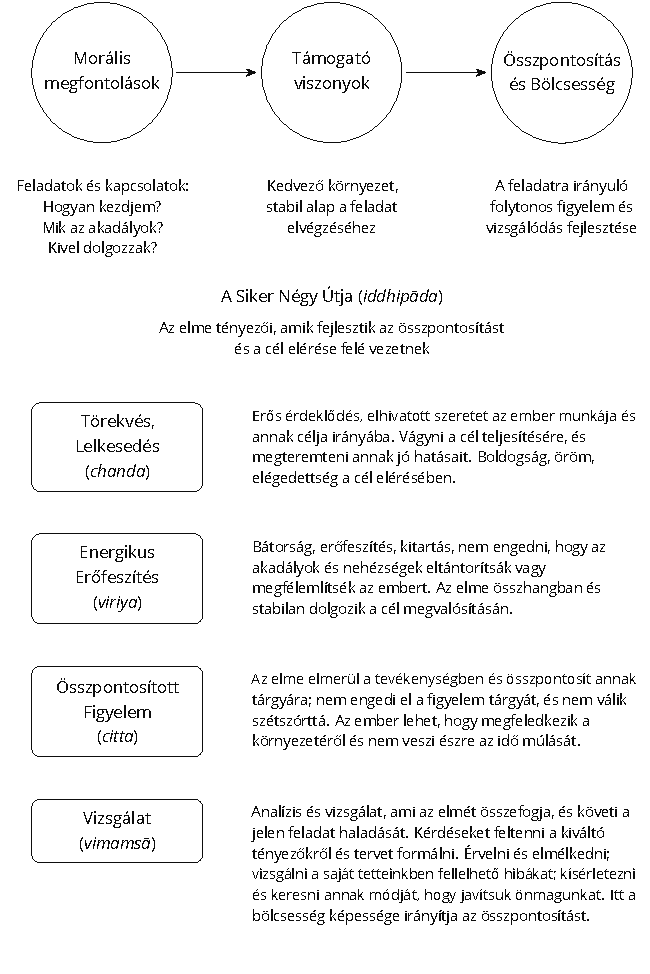
\includegraphics[width=0.95\linewidth]{./manuscript/tex/diagrams/paths-to-success-hu.pdf}
\end{figure}

\clearpage
\normalpagelayout

A csendes és nyugodt időszakok áldásnak számítanak. Mindig is értékeltem
egy stabil rutint, ami hosszú időszakokat enged a koncentrált munkára
vagy intenzív gyakorlásra. Más részről, akadályok és konfliktusok is
garantáltan jönni fognak.

Nem kell amiatt aggódnunk, hogy a meditáció meg fogja oldani minden
problémánkat, és nem lesz mit tennünk. A meditáció nem
probléma-megoldás. Ez az éberség olyan gyakorlása, ami túljut a belső
akadályokon és szembe néz a külső problémákkal, ahogy azok elénk
kerülnek. Ha egy fontos ügyet kell elintéznünk, segít, ha előbb
kitisztítjuk a fejünket. Viszont pusztán az, hogy ülünk a párnán mintha
túlhaladtunk volna minden problémán, a jelenre való tudatlanságot
gyakoroljuk, nem a tudatosságot.

Szándékosan szembe nézni és jó képességgel megbirkózni ezekkel arany
esélyt ad arra, hogy az elme képzését a korábbi korlátokon túl
fejlesszük. A zavaros káosz gazdag a lehetőségekben, hogy gyakorlati
úton fejlődjünk és tanuljunk.

Nem magukat az érzéseket keressük, nem különleges érzéseket próbálunk
létrehozni a meditációval, nem azt a helyzetet keressük, ahol mindig
minden jól megy nekünk. A kellemes, kellemetlen, semleges érzések
önmagukban nem adnak nekünk helyes megértést, ha követjük a befolyásukat
és gépiesen reagálunk rájuk. Az éberségnek észre kell vennie az
állandótlanságukat és bizonytalanságukat. Akkor megértéssel látjuk mi a
jótékony, és mi a kártékony a jelen helyzetben.

\keywords{csónak a folyón, én és enyém}

Könnyű a meditációt gyakorolni, vagy nehéz? Egy hasznos kép amire
gondolhatunk, ahogy egy csónak halad a folyón. Amikor a csónak áruval
töltött ládákkal van megrakva, a sok teher alatt nehezen és lassan
halad. Épp, hogy a víz felett tudja tartani magát.

Azt szeretnénk, hogy a csónakunk gyorsan haladjon, nem igaz? De
ugyanakkor ragaszkodunk mindenhez amivel megraktuk. Könnyítenünk kell a
csónakon, elengedni az `én' nehéz súlyát. Mi hozzuk létre az `én' és
`enyém' terhét. Mi hozzuk létre a benyomást, hogy `ilyen voltam, ilyen
vagyok, ilyen kell legyek'. `Az az enyém volt, ez az enyém, ez meg
akarom tartani, azt meg kell szereznem'. Ez a súly húzza le a csónakot.

Az érzés, hogy elég, ami van, megteremti a teret a nagylelkűségre. Az
elégedettség a gyakorlás folyamatos része, nem egy rögzült, feltételhez
kötött állapot. A tettek és a tanulás mint egy patak folynak az
elégedettségből. Mikor azt gondolom, `kész leszek elkezdeni, mikor már
megvan a \ldots{}', az elégedetlenség köti le a gondolataimat és folyton
megszakítja a koncentrációmat a jelen helyzetre.

\keywords{jótékony gondolatok, béke}

Viszont amikor azt gondolom, `nem vagyok jó ebben, de ennyi is elég,
hogy elkezdjem', elfogadni a jelen határaimat energiát ad a cselekvésre.
Végül gyakran többet is tudok tenni mint képzeltem.

A gondolkodás rossz hírnevet kap a meditációs könyvekben, de a tiszta
gondolatok megalapozzák a feltételeket a helyes hozzáállás fejlődéséhez.
Az elharapózó, kényszeres gondolkodás valóban fájdalmas tapasztalat, de
ha meg akarunk állítani minden gondolatot, mellé lövünk a célnak.

Vedd észre, hogy a jótékony gondolatokat megelégedettség és béke követi.
Erkölcsös tetteinket tudatosan felidézve kialakul a stabilitás és
ön-tisztelet érzete. Bízunk magunkban, hogy elengedjük ami fölösleges,
mert érezzük, hogy ami van az már elég.

Ha fejben akarjuk megoldani, a gyakorlás gyorsan bonyolulttá válik. A
meditációban, a testen keresztüli éberség egy megbízható irány: Az
érzéseket és elme állapotokat figyeljük, ahogy jönnek és mennek,
nézőpontunkat áthelyezzük, és nem magunkkal vagyunk elfoglalva. A
bonyolult kérdéseket magunk mögött tudjuk hagyni, mert már nincs
szükségünk a válaszokra.

\keywords{könnyű csónak, élvezetes tanulás}

Mi teszi lehetővé, hogy tovább tanuljunk és fejlődjünk? Az utazás akkor
a legélvezetesebb, amikor a horizont egyre tovább tágul, a korábbi
korlátainkon túl. A horizontot nem azzal tágítjuk, hogy messzire
utazunk, hanem azzal, hogy új szemmel látunk. A vágy, hogy megtartsuk
azt, amiről azt gondoljuk mi vagyunk, határozza meg a jelen korlátunkat.

A csónak könnyű, amikor üres az éntől és enyémtől. Nagy távolságokat
tesz meg dráma és zaj nélkül. Mi történik, ha a csónakban ülünk, és
valaki a csónakjával nekünk ütközik? Rákiáltunk, ellökjük az evezővel,
és egész nap erről panaszkodunk. Ez mind lehet, hogy jogos, de tönkre
tettük a napunkat a saját rossz társaságunkkal. Nehéz ebben a
bölcsességet látni. Mi történik, ha egy üres csónak ütközik nekünk?
Honnan eredt a korábbi harag és negatív indulat?

Hajlamosak vagyunk az én és enyémről szóló történeteket gyártani, akár
valós, akár képzeletbeli események alapján. Ha komolyan vesszük ezeket,
és valóságot adunk nekik, a történetek kezdenek irányítani minket, és
korábban nem létező problémákat hozunk létre.

\enlargethispage*{\baselineskip}

Előfordul, hogy ülünk a meditációs párnán, és vitákat kezdünk eljátszani
a képzelet bábjaival. Komoly az ügy, nekünk kell nyerni! Módszeresen
végig gondolni egy problémát hasznos eszköz, de önmagunk felé irányuló
szimpátiára és kedvességre is szükség van az építő jellegű belső
bárbeszédhez. Másként, amikor az én magával beszél, rossz társaságban
találja magát.

\keywords{aki tud önmagán nevetni}

Meglepő, mennyire fel tudjuk húzni magunkat egy olyan helyzettel
kapcsolatban, ami még meg sem történt. Segít, ha tartunk egy csipet
humort az oldal zsebünkben, vészes komolyság esetére. A görög filozófus,
Epiktétosz mondását felidézve, `Aki tud önmagán nevetni, sosem fogy ki a
nevetni valóból.'

\keywords{az érzékek egyszerűsége, elengedés}

A meditáció gyakorlásában visszaálltjuk a helyes szemléletet azzal, hogy
visszatérünk az érzékek egyszerűségéhez. A történeteket, ha vannak, a
változó körülmények nézőpontjából szemléljük. Az érzékek vizsgálatával
egy alapvetőbb valóságra alapozzuk a figyelmünket. A kellemes érzet
ilyen, ahogy most tapasztaljuk, a kellemetlen érzet ilyen, a semleges
érzet ilyen, kezdete van és vége, változik és üres.

A gyakorlásban nem az lesz értékes, hogy sietve eredményeket halmozunk
fel, hanem, hogy teret hagyunk az elengedésnek és türelemnek. Van amikor
cselekedni kell, de meglepően sokféle nehézséget megold az egyszerű
türelem. A sértettség vagy sürgető fontosság érzése magunkból ered. A
visszafogottság biztonságos nézőpontot nyújt ilyenkor, magunkkal és
másokkal szemben is. Engedjük a csónakunkat csendben tovább úszni.
